\section{Task 4: Less or More?}
\label{sec:task4}

\subsection{Results for 50 L and 25000 L}
\label{sec:task4-results}

The amber-beer optimisation is repeated for 50 L, 5000 L, and 25000 L. The relaxation, rounded-process solution, and MILP solution have the same costs for these three cases because the relaxed process variables are already integral.

\begin{table}[H]
\renewcommand{\arraystretch}{1.15}
\caption{Task 4 Volume Comparison}
\label{tab:task34-volume-comparison}
\centering
\small
\begin{tabular}{@{}rrrrr@{}}
\toprule
Beer volume (L) & Relaxation cost & Rounded cost & MILP cost & MILP cost per litre \\
\midrule
50 & 67.767 & 67.767 & 67.767 & 1.355 \\
5000 & 4497.687 & 4497.687 & 4497.687 & 0.900 \\
25000 & 13420.213 & 13420.213 & 13420.213 & 0.537 \\
\bottomrule
\end{tabular}
\end{table}

The corresponding MILP process choices are $(0,0)$ for 50 L, $(0,1)$ for 5000 L, and $(1,1)$ for 25000 L. Thus, the smallest batch can be produced without activating malting or mashing, the 5000 L case uses mashing only, and the largest batch uses both malting and mashing.

The 5000 L ingredient solution is already reported in Task 3. Tables~\ref{tab:task34-solution-summary} and~\ref{tab:task34-nonzero-ingredients} therefore give the additional MILP solution details for 50 L and 25000 L. The quality values are reported for completeness, but they are not constrained in this task.

\begin{table}[H]
\renewcommand{\arraystretch}{1.15}
\caption{Task 4 MILP Solution Summary for Additional Volumes}
\label{tab:task34-solution-summary}
\centering
\small
\begin{tabular}{@{}rcrrrrr@{}}
\toprule
Volume (L) & Process & Cost & EBC & $Q_S$ & $Q_H$ & $Q_Y$ \\
\midrule
50 & $(0,0)$ & 67.767 & 29.000 & 1.000 & 1.000 & 1.000 \\
25000 & $(1,1)$ & 13420.213 & 20.000 & 1.000 & 1.000 & 1.000 \\
\bottomrule
\end{tabular}
\end{table}


\begin{table}[H]
\renewcommand{\arraystretch}{1.12}
\caption{Task 4 Non-Zero Ingredients for 50 L and 25000 L}
\label{tab:task34-nonzero-ingredients}
\centering
\small
\begin{tabular}{@{}rllr@{}}
\toprule
Volume (L) & Group & Variable & Amount (kg) \\
\midrule
50 & Malt extract & \texttt{maltextract04} & 0.721 \\
50 & Malt extract & \texttt{maltextract10} & 6.911 \\
50 & Hops & \texttt{hop07} & 0.068 \\
50 & Yeast & \texttt{yeast05} & 0.037 \\
25000 & Barley & \texttt{barley04} & 799.499 \\
25000 & Barley & \texttt{barley09} & 5560.150 \\
25000 & Hops & \texttt{hop07} & 34.211 \\
25000 & Yeast & \texttt{yeast05} & 18.750 \\
\bottomrule
\end{tabular}
\end{table}


\subsection{Marked Costs on Task 1 Plot}
\label{sec:task4-marked-plot}

The three production volumes from Table~\ref{tab:task34-volume-comparison} are marked on the cost-volume plot from Task 1.

\begin{figure}[H]
\centering
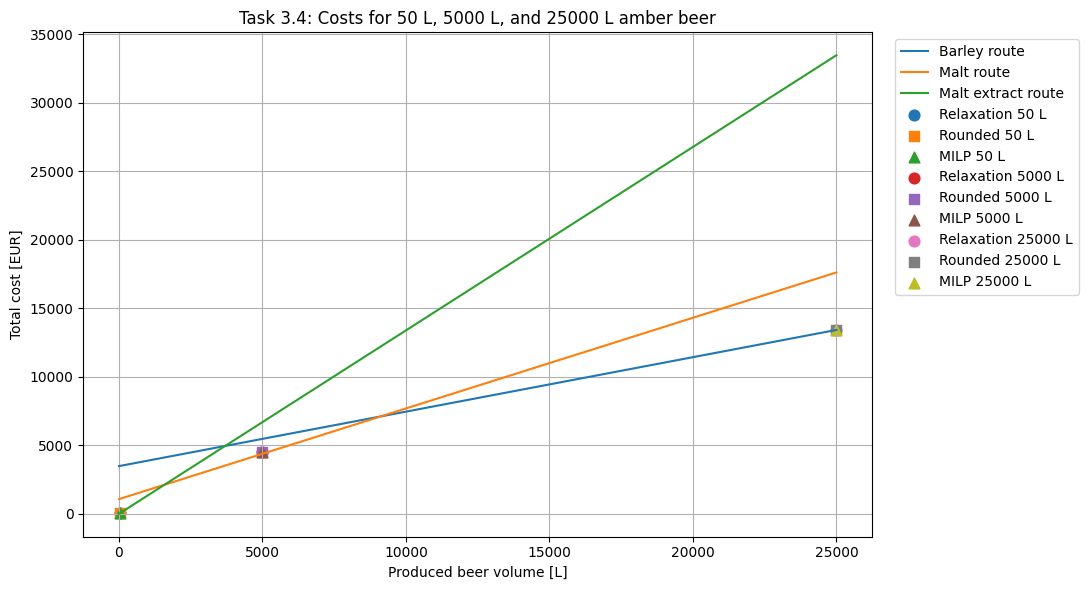
\includegraphics[width=\linewidth]{bilder/task_34_marked_costs.png}
\caption{Task 4 costs for 50 L, 5000 L, and 25000 L marked on the Task 1 cost-volume plot.}
\label{fig:task34-marked-costs}
\end{figure}

The marked points follow the combined minimum-cost curve from Task 1. This is expected because the optimal source route changes with volume as fixed process costs become less important relative to variable ingredient costs.

\subsection{Cost per Litre Discussion}
\label{sec:task4-discussion}

The cost per litre decreases as the production volume increases. The 50 L batch is expensive per litre because any fixed process cost is spread over very few litres. Larger batches spread fixed costs over more output, so the cost per litre is lower. The 25000 L case has the lowest cost per litre in Table~\ref{tab:task34-volume-comparison}.
